\documentclass{article}
\usepackage{hyperref}
\usepackage[MeX]{polski}
\usepackage{parskip}
\usepackage[utf8]{inputenc}
\usepackage{graphicx}
\title{Projekt -- Programowanie Aplikacji Internetowych}
\author{\textsc{Paweł Sołtysiak I1-41A} \\ \texttt{psoltysiak@wi.zut.edu.pl}}

\begin{document}
\maketitle

\section{Opis}
Aplikacja internetowa, Messim służy do komunikacji pomiędzy użytkownikami serwisu, a także służy oceniania i wybierania najlepszych obrazków zgromadzonych przez użytkowników.

Aplikacja posiada możliwość rejestracji oraz logowania się użytkownika. Następnie zalogowany użytkownik posiada możliwość wgrywania obrazków na serwer poprzez formularz. Oprócz załączonego obrazka użytkownik może dodać wiadomość tekstową, która jest dołączona do jego obrazka. Kolejną możliwością serwisu jest ocenianie obrazków dodanych do serwisu. Każdy użytkownik może oddać swój głos pod obrazkiem, jego sumaryczna ilość zebrana pod obrazkiem.

Pod każdym obrazkiem inni użytkownicy serwisu mogą odpowiedzieć na wysłany obrazek.


\section{Prezentacja działania aplikacji}
Strona główna dla użytkownika niezalogowanego

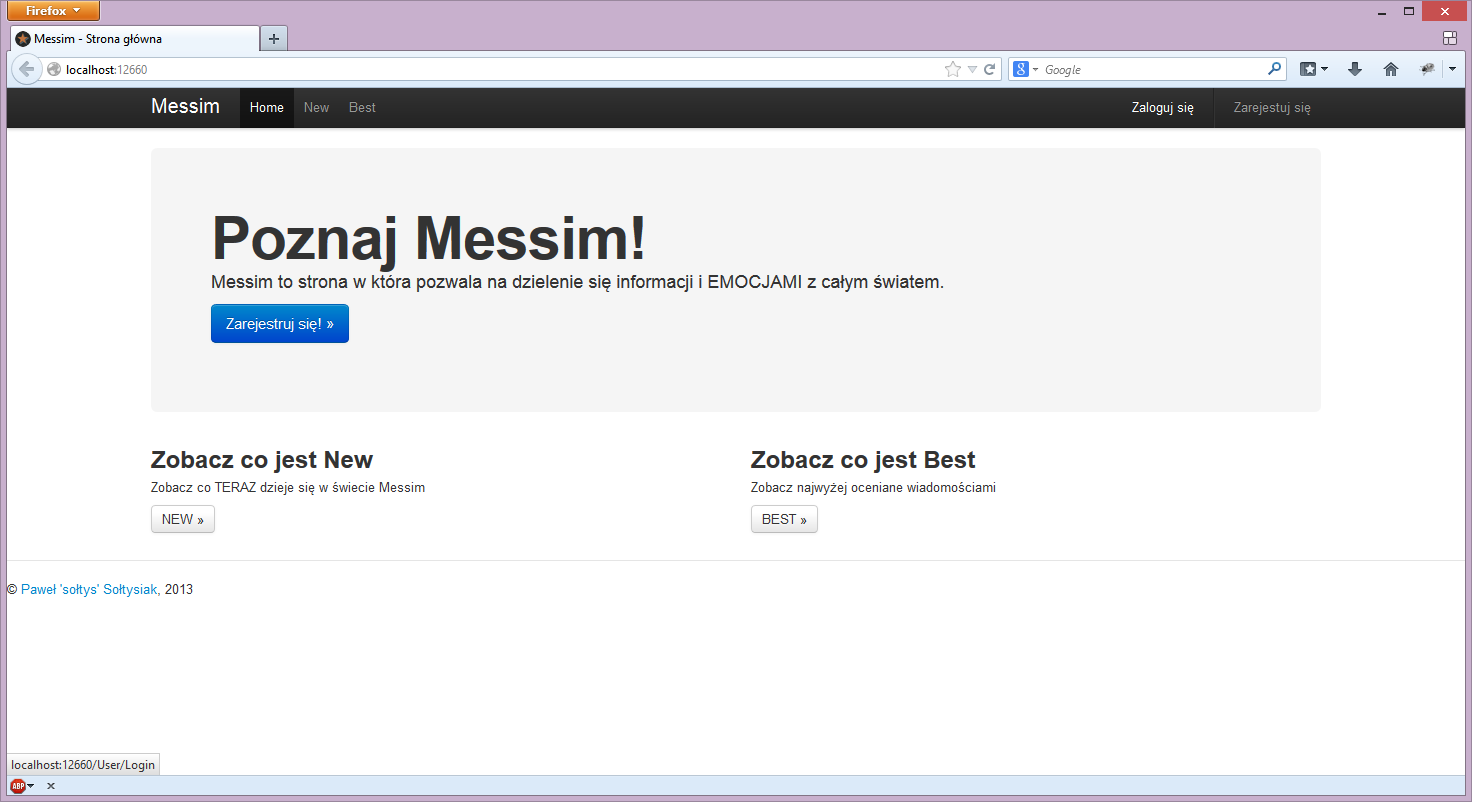
\includegraphics[width=\textwidth]{screenshots/home_page_not_singup}

Formularz rejestracji

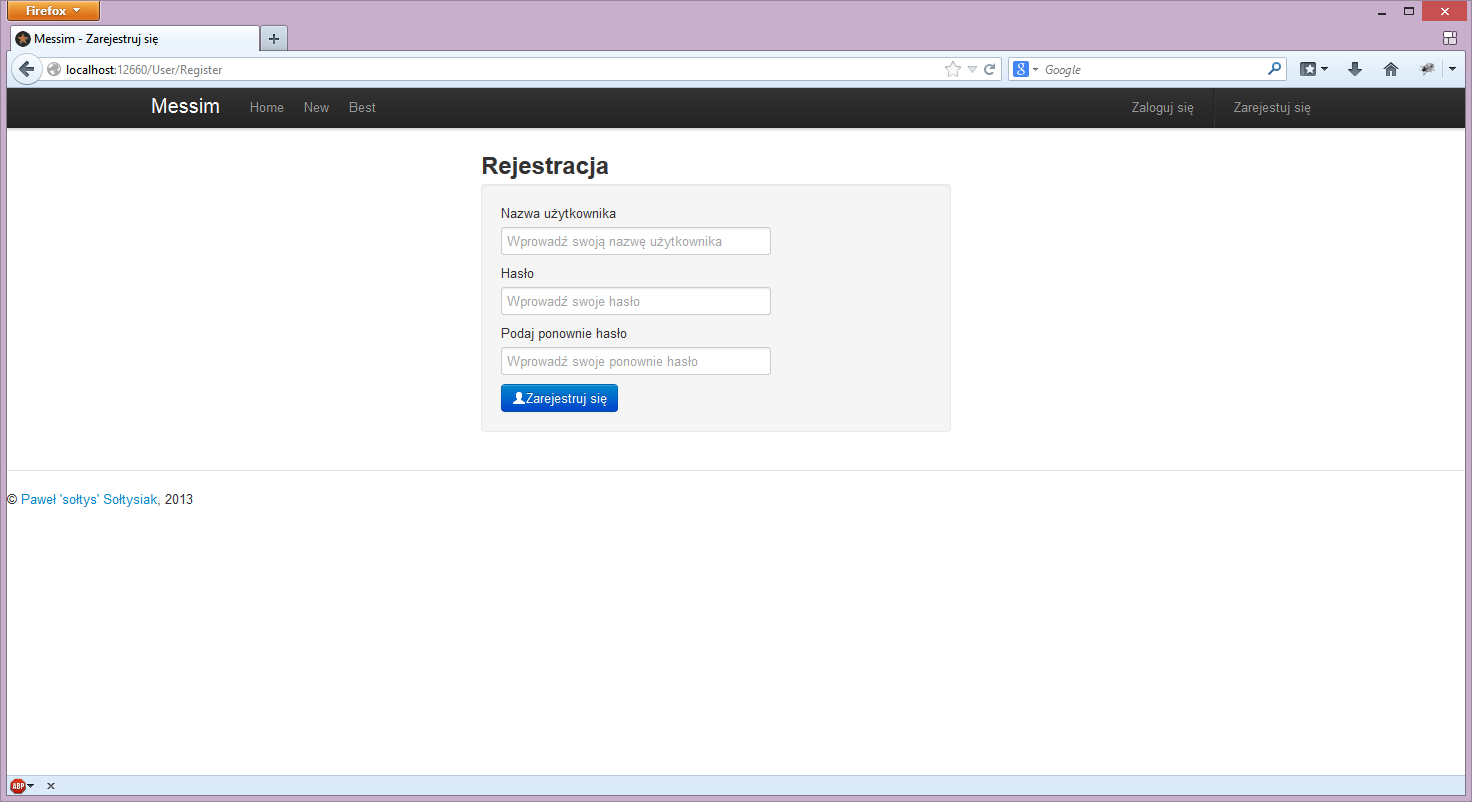
\includegraphics[width=\textwidth]{screenshots/register_page}

Strona główna dla użytkownika zalogowanego

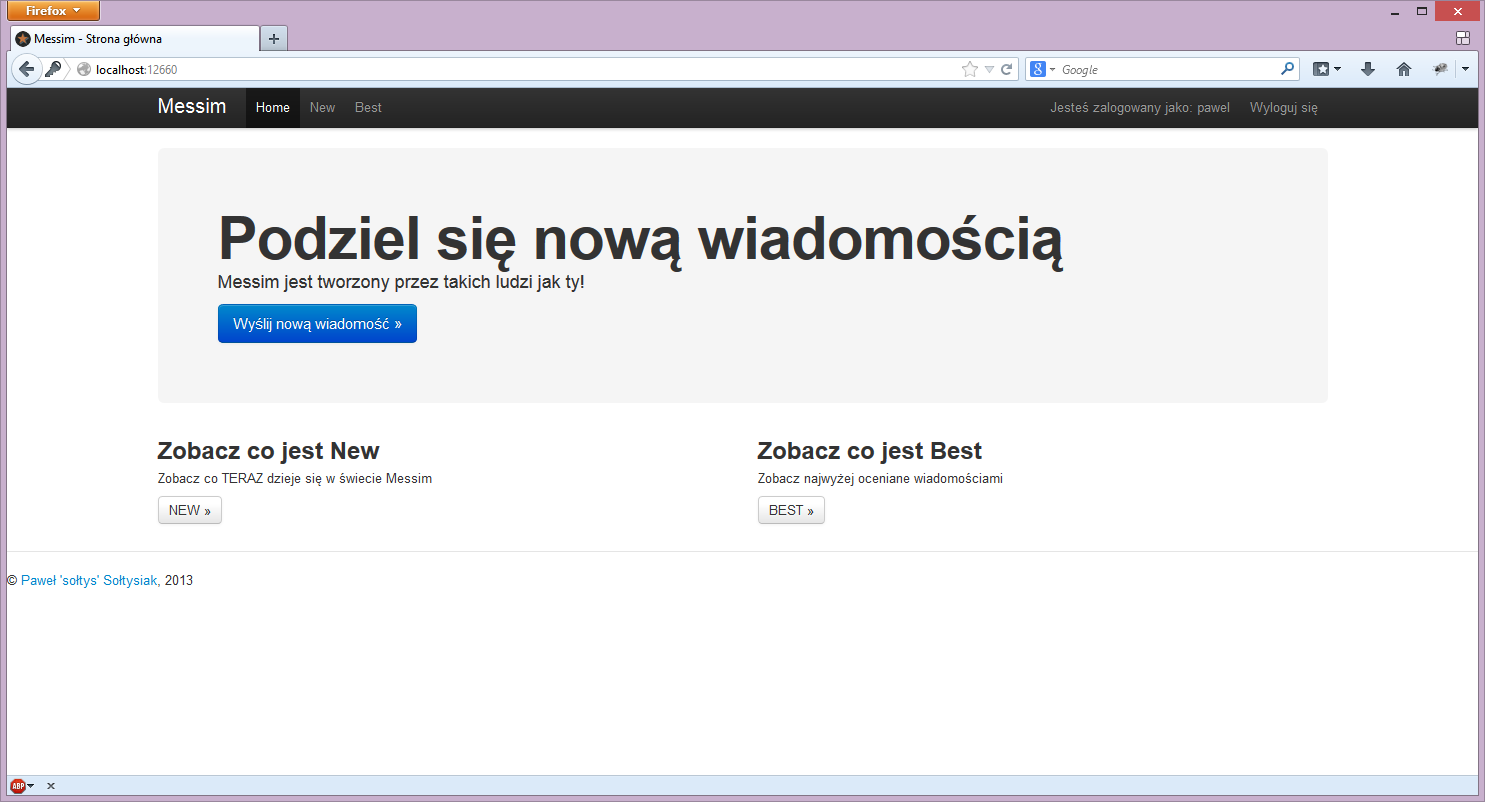
\includegraphics[width=\textwidth]{screenshots/home_page_with_user}

Formularz do przesyłania wiadomości i zdjęć

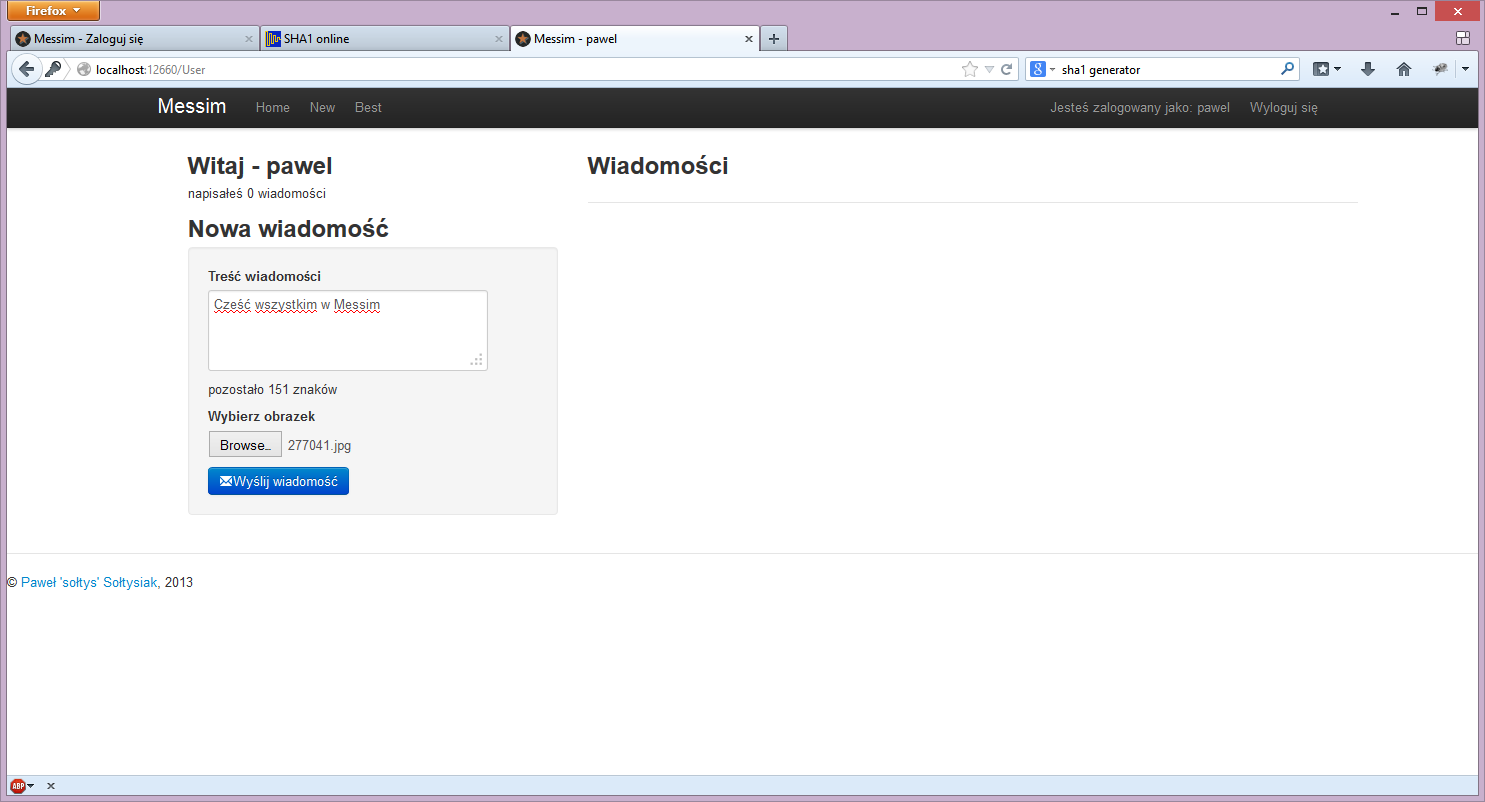
\includegraphics[width=\textwidth]{screenshots/posting_first_image}

Profil osoby po wysłaniu zdjęcia

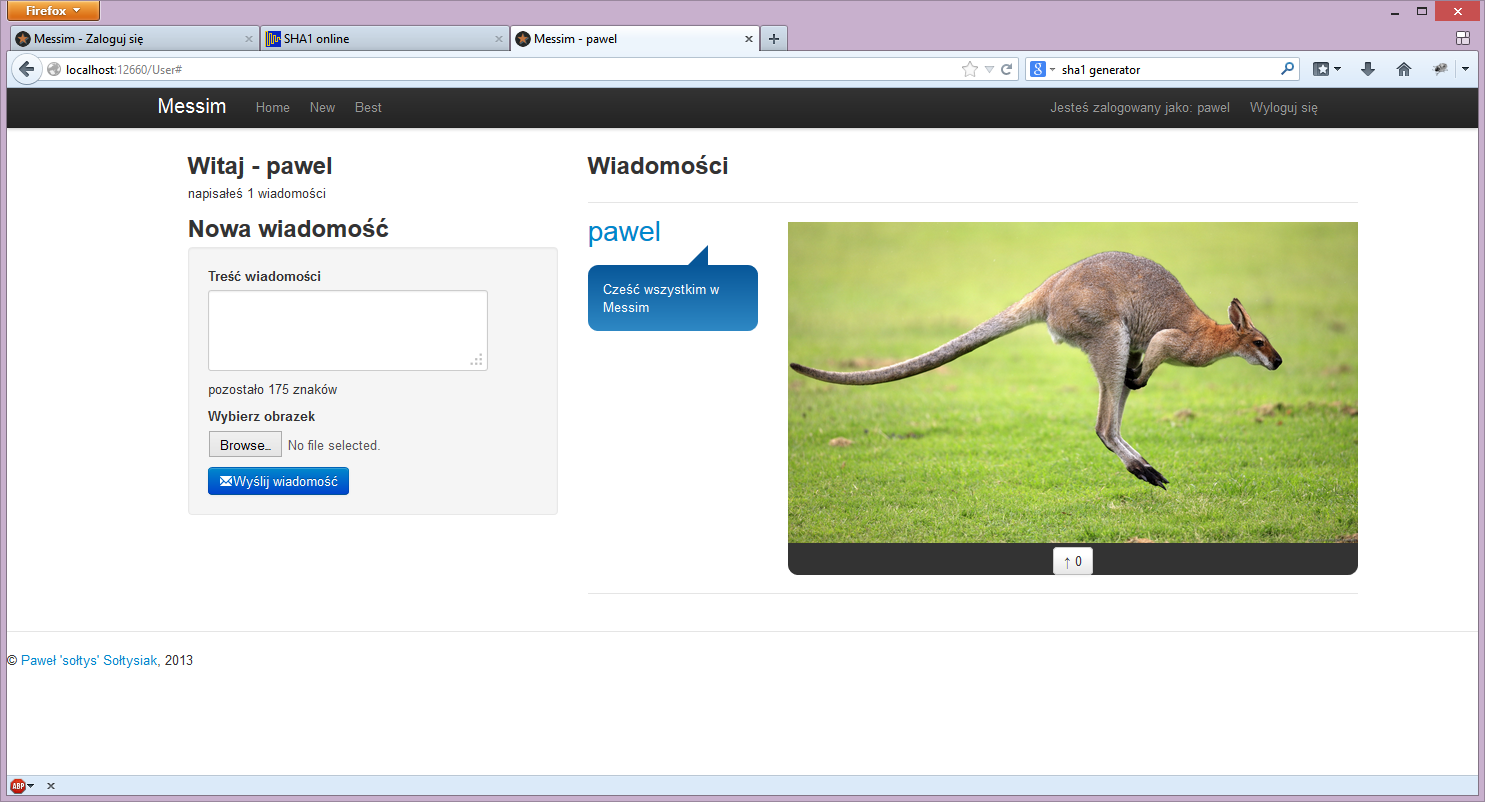
\includegraphics[width=\textwidth]{screenshots/posted_first_image}

\section{Opis technologiczny}
\begin{itemize}
\item Język programowania \texttt{C\#}
\item .NET Framework 4.0
\item ASP.NET MVC 3.0
\item SQL Server 2010
\item Entity Framework
\item NUnit
\end{itemize}

Kod źródłowy dostępny pod adresem \url{http://github.com/soltys/Messim}
\section{Informacje dodatkowe}
Aplikacja była tworzona z myślą o pokazaniu jej na tzw. "Nocy z Microsoft". Impreza była organizowana w Warszawie, gdzie zostały zaproszone grupy studenckie .NET z całego kraju.

\end{document}

